\documentclass{article}
\usepackage[utf8]{inputenc}
\usepackage[spanish, es-tabla]{babel}
\usepackage[a4paper]{geometry}
\usepackage{graphicx}
\usepackage{booktabs} 
\usepackage[table]{xcolor}
\usepackage{amsmath}
\usepackage{float}
\usepackage{hyperref}

\usepackage{dcolumn}
\newcolumntype{L}{D{.}{.}{1.1}}

\spanishdecimal{.} 

\usepackage{listings}
\usepackage{color}
\definecolor{dkgreen}{rgb}{0,0.6,0}
\definecolor{gray}{rgb}{0.5,0.5,0.5}
\definecolor{mauve}{rgb}{0.58,0,0.82}
\lstset{ 
  language=R,                     % the language of the code
  basicstyle=\footnotesize,       % the size of the fonts that are used for the code
  numbers=left,                   % where to put the line-numbers
  numberstyle=\tiny\color{gray},  % the style that is used for the line-numbers
  stepnumber=1,                   % the step between two line-numbers. If it's 1, each line
                                  % will be numbered
  numbersep=5pt,                  % how far the line-numbers are from the code
  backgroundcolor=\color{white},  % choose the background color. You must add \usepackage{color}
  showspaces=false,               % show spaces adding particular underscores
  showstringspaces=false,         % underline spaces within strings
  showtabs=false,                 % show tabs within strings adding particular underscores
  frame=single,                   % adds a frame around the code
  rulecolor=\color{black},        % if not set, the frame-color may be changed on line-breaks within not-black text
  tabsize=2,                      % sets default tabsize to 2 spaces
  captionpos=b,                   % sets the caption-position to bottom
  breaklines=true,                % sets automatic line breaking
  breakatwhitespace=false,        % sets if automatic breaks should only happen at whitespace
  title=\lstname,                 % show the filename of files included with \lstinputlisting;
                                  % also try caption instead of title
  keywordstyle=\color{blue},      % keyword style
  commentstyle=\color{dkgreen},   % comment style
  stringstyle=\color{mauve},      % string literal style
  escapeinside={\%*}{*)},         % if you want to add a comment within your code
  morekeywords={*,...}            % if you want to add more keywords to the set
} 

\geometry{top=2.0cm, bottom=3.0cm, left=2.5cm, right=2.5cm}
\title{Algoritmos Bioinspirados: Evolución Diferencial}
\author{Alberto García y Diego Martínez}

\begin{document}
\maketitle
En este trabajo hemos implementado la opción T3\_DE, correspondiente al algoritmo de evolución diferencial desarrollado en el artículo de Tian, Gao y Dai \cite{mainPaper}. Este informe contiene en sus secciones, la descripción del algoritmo, un resumen de los problemas a resolver, la estructura y los parámetros del experimento, los resultados y conclusiones, las referencias y un anexo con el código del programa.

\section{Descripción del Algoritmo}
Este algoritmo es de tipo evolutivo, luego su esquema general será el siguiente. Crearemos un conjunto de \textbf{mutaciones}, haremos un \textbf{crossover} entre la población de padres y las mutaciones para crear una nueva población de hijos, y realizaremos una \textbf{selección} para seleccionar los mejores mejores individuos entre la población de padres e hijos.

En concreto este algoritmo es de evolución diferencial, lo que quiere decir que la estrategia para las mutaciones está basada en diferencias entre individuos. Esto implica que la elección individuos más o menos ``buenos'' para calcular estas diferencias contribuye a que el algoritmo tenga un comportamiento más convergente o más exploratorio. En concreto, este algoritmo tiene un modelo híbrido con algunos parámetros autoadaptativos, de forma que especialmente en las en primeras generaciones y cuando el porcentaje de hijos que suceden a los padres es bajo, los parámetros se adaptan para ofrecer un mayor comportamiento exploratorio.

\subsection{Mutación}
La mutación para cada individuo en una generación se genera con una estrategia rand-to-guiding (exploratoria) o current-to-guiding (convergente), la cual se selecciona por sorteo con una umbral de probabilidad $\xi_1$. A estas estrategias se les añade una segunda componente extra que dependiente de un cierto $\vec{d}_{r2, G}$, el cual pretende añadir un elemento de aleatoriedad a la mutación. La expresión para la mutación queda de la siguiente manera:
\begin{equation}
    \vec{v}_{i,G} = \left\{\begin{array}{ll}
            \vec{x}_{\text{rand},G} + F_1(\vec{x}_{g,G}-\vec{x}_{\text{rand}, G})+ F_2(\vec{x}_{r1,G}-\vec{d}_{r2, G})&\text{si rand}<\xi_1,\\
            \vec{x}_{\text{cur},G} + F_1(\vec{x}_{g,G}-\vec{x}_{\text{cur}, G})+ F_2(\vec{x}_{r1,G}-\vec{d}_{r2, G})&\text{caso contrario},
    \end{array}\right.
\label{ec_mutacion}
\end{equation}
donde las variables son:
\begin{itemize}
    \item $\xi_1$: Umbral de probabilidad para la selección de estrategias. (Constante entre 0 y 1)
    \item rand: Variable aleatoria con probabilidad uniforme entre 0 y 1.
    \item $G$: Generación del individuo.
    \item $\vec{v}_{i,G}$: Mutación para el individuo $i$.
    \item $\vec{x}_{\text{cur},G}$: Individuo $i$ para el que queremos crear la mutación. (Current individual)
    \item $\vec{x}_{\text{rand},G}$, $\vec{x}_{\text{r1},G}$: Individuos aleatorios. ($\vec{x}_{\text{rand},G}\neq\vec{x}_{\text{cur},G}$, $\vec{x}_{\text{r1},G}\neq\vec{x}_{\text{cur},G}$)
    \item $\vec{x}_{g,G}$: Individuo seleccionado entre la élite de la generación. (Guiding individual)
    \item $F_1$: Peso de la estrategia principal. (Parámetro entre 0 y 1)
    \item $F_2$: Peso de la componente puramente aleatoria. (Constante entre 0 y 1)
    \item $\vec{d}_{r2,G}$ Vector aleatorio dentro del espacio de búsqueda.
\end{itemize}

Hemos visto que la expresión anterior para la mutación requiere tres componentes que hay que determinar en cada generación. Estos son el guiding individual $\vec{x}_{g,G}$, el parámetro $F_{2}$ y el vector aleatorio $\vec{d}_{r2,G}$.\vspace{1cm}

\underline{Guiding Individual $\vec{x}_{g,G}$}: Se elegirá de manera equiprobable entre los elementos de $\text{Pop}_{s}$ o bien $\text{Pop}_{g}$, donde la elección de un conjunto u otro se decidirá de si un parámetro llamado Success Ratio de la generación, $SR_{G}$ sobrepasa un cierto umbral constante $\xi_{3}$ entre 0 y 1. El Success Ratio se define como $SR_{0}=1$ y para el resto $SR_{G}=NS_{G}/NP$, es el número de hijos que suceden a los padres en la generación entre el número total de la población. La expresión entonces es la siguiente:
\begin{equation}
    \vec{x}_{g,G} \text{ seleccionado aleatoriamente de } = \left\{\begin{array}{ll}
            \text{Pop}_{s} & \text{si }SR_{G-1}<\xi_3,\\
            \text{Pop}_{g} & \text{caso contrario},
    \end{array}\right.
\label{guiding}
\end{equation}
donde $\text{Pop}_{s}$ es el top $floor((1-t^{3})\times 100)\%$ de la población, con $t=G/G_{\max}$ y $G_{\max}$ número máximo de generaciones; y $\text{Pop}_{g}$ es el top $10\%$ de la población. Como $\xi_{3}$ acostumbra a ser pequeño (0.05), si ha habido poco reemplazo se seleccionará el guiding individual de $\text{Pop}_{s}$, el cual empieza siendo toda la población y a medida que avanzan las generaciones es cada vez más elitista. Luego si al principio el condicionamiento ha sido muy bueno y la tasa de reemplazos en las primeras generaciones es baja, la selección del guiding individual se hará sobre un conjunto muy grande de la población aumentando las posibilidades de seleccionar un ``peor'' individuo mejorando la exploración.\vspace{1cm}

\underline{Parámetro $F_{1}$}: Este parámetro corresponde al peso que se le da al vector de cambio $\vec{x}_{g,G}-\vec{x}_{\text{cur}, G}$, por lo que su valor dependerá de dos escenarios.

\begin{itemize}
    \item Si el fitness del guiding individual es mejor que el del current individual, entonces $\vec{x}_{g,G}-\vec{x}_{\text{cur}, G}$ es una dirección prometedora. El peso $F_{1}$ será proporcional a cuan mejor es el fitness del guiding individual respecto su generación:
\begin{equation}
	F_{1}=\dfrac{1}{2}\left(1+\dfrac{f_{\max}-f_{g}}{f_{\max}-f_{min}}\right),
	\label{F1_Pos}
\end{equation}
donde $f_{\max}$, $f_{min}$, $f_{g}$ son el fitness del máximo, el mínimo y el guiding individual de la generación respectivamente.
    \item Si el fitness del guiding individual es peor que el del current individual, entonces $\vec{x}_{g,G}-\vec{x}_{\text{cur}, G}$ no es una dirección prometedora. Tomaremos la dirección opuesta como dirección prometedora haciendo que $F_{1}$ sea:
\begin{equation}
    F_{1} = \left\{\begin{array}{ll}
            -0.05 & \text{si }-randn>-0.5,\\
            -0.95 & \text{si }-randn<-0.95,
    \end{array}\right.
\label{F1_neg}
\end{equation}
donde $randn$ es una variable aleatoria normal con $\mu=0.5$ y $\sigma=0.2$.
\end{itemize}

\underline{Vector aleatorio $\vec{d}_{r2,G}$}: La estrategia para crear este vector aleatorio es elegir un individuo aleatorio de la población y sortear para cada una de sus componentes con un cierto umbral $\xi_2$, si se sustituye la componente por un elemento aleatorio dentro del espacio de búsqueda. Esto es:

\begin{equation}
    \vec{d}^{j}_{r2,G} = \left\{\begin{array}{ll}
            L^{j} + rand(0,1)\times(U^{j}-L^{j})&\text{si }rand(0,1)<\xi_2,\\
            \vec{x}_{\text{r2},G}&\text{caso contrario},
    \end{array}\right.
\label{ec_rand_vec}
\end{equation}
\begin{itemize}
    \item $\xi_{2}=(1+9\times 10^{5(t-1)})/100$: Umbral de probabilidad para la selección aleatoria.
    \item rand(0,1): Muestreo aleatorio de una uniforme entre 0 y 1.
    \item $\vec{x}_{\text{r2},G}$: Individuo aleatorio. ($\vec{x}_{\text{r2},G}\neq\vec{x}_{\text{r1},G}$)
    \item $L^{j}$: Cota inferior de la componente $j$-ésima en el espacio de búsqueda.
    \item $U^{j}$: Cota superior de la componente $j$-ésima en el espacio de búsqueda.
\end{itemize}
Vemos que por la definición de $\xi_{2}$, y recordando la definición de $t=G/G_{\max}$ dada en el guiding individual, está comprendida entre 0 y 1. De hecho este parámetro es monótono decreciente, y en las primeras generaciones es cercano a 1 y en la última igual a 0. Eso hace que capacidad de obtener una componente puramente aleatoria y diferente a un individuo de la población muy alta al principio (explora) y muy baja al final (converge) que sería un comportamiento deseable.

\subsection{Crossover}
Mediante el crossover generamos nuevos individuos que comparen características entre la población inicial y difieren en alguna mutación. Lo primero que hacemos es definir la probabilidad $CR$ de que un individuo de la siguiente generación herede características del individuo mutado.
\begin{equation}
    \text{CR} = 1 - \frac{R_g}{\text{NP}},
    \label{ec_CR}
\end{equation}
con
\begin{itemize}
    \item NP: Número total de individuos.
    \item $R_g$: Ranking del guiding individual. En el conjunto ordenado de individuos por fitness, el puesto que ocupa el guiding individual respecto al mejor.
\end{itemize}
Si nos fijamos en la ec.\eqref{ec_mutacion} vemos que las mutaciones tienen tendencia a acercarse al guiding individual. El crossover explota esto otorgando una $CR$ alta cuando el fitness del guiding individual es ``mejor"" ($R_g$ pequeño).

Una vez calculada la probabilidad de mutación $CR$ generamos un individuo mutado o \textit{trial} a partir de cada par individuo original - mutación. Hacemos que el \textit{trial} $u_{i,G}$ herede componentes de la mutación en función del $CR$:
\begin{equation}
    u_{i,G}^j = \left\{\begin{array}{ll}
        v_{i,G}^j&\text{si rand}\le\text{CR ó randn}(i)=j,\\
        x_{i,G}^j&\text{otro caso},
        \end{array}\right.
    \label{ec_crossover}
\end{equation}
donde el superíndice $j$ denota la $j$-ésima componente, y
\begin{itemize}
    \item randn$(i)$: Entero aleatorio entre 1 y $D$, siendo $D$ el número de componentes de $x, v, u$.
\end{itemize}
La condición randn$(i)=j$ asegura que al menos una componente (la componente número rand$(i)$) sea mutada. Nótese que para problemas de una única dimensión esta condición siempre se cumple y los \textit{trials} son idénticos a la población mutada.
\subsection{Selección}
En esta parte del algoritmo se elige al individuo de la generación $G+1$, eligiendo para ello entre el individuo de la generación $G$ y el trial generado a partir de él.

Para efectuar esta selección se define previamente un fitness ponderado:
\begin{equation}
    f_w(x_{i,G}) = \alpha\frac{f(x_{i,G}) - f_\text{min}}{f_\text{max} - f_\text{min}} + (1-\alpha)\frac{\text{Dis}_\text{max} - \text{Dis}(x_{i,G}, x_{best,G})}{\text{Dis}_\text{max} + \text{Dis}(x_{i,G}, x_{best,G})}
    \label{ec_fitness_ponderado}
\end{equation}
Con
\begin{itemize}
    \item $f_w$: Función \textit{fitness} ponderada.
    \item $f, f_\text{min}, f_\text{max}$: Función \textit{fitness} del problema a resolver; el mínimo y el máximo valor de esta función para la población de la generación $G$.
    \item $\alpha$: Variable aleatoria entre 0.8 y 1.
    \item Dis, Dis$_\text{max}$: Función que devuelve la distancia euclídea entre dos puntos; la máxima de estas distancias para la generación actual.
    \item $x_{\text{best}, G}$: Individuo con mejor \textit{fitness} en la generación $G$.
\end{itemize}
La función fitness ponderada introduce una penalización por alejarse del individuo con mejor \textit{fitness}.

El método de selección es esencialmente comparar ambos los \textit{fitness} de el individuo original y el trial. Si el trial supera al original el individuo es sustituido por el trial.
\begin{equation}
    \vec{x}_{i,G+1} = \left\{\begin{array}{cl}
            \vec{u}_{i,G}&\text{si }f(\vec{u}_{i,G})<f(\vec{x}_{i,G})\\
            \vec{u}_{i,G}&\text{si }f(\vec{u}_{i,G})\le f(\vec{x}_{i,G})\text{ y }x_{i, G}\neq x_{\text{best}, G}\\
            \vec{x}_{i,G}&\text{otro caso}
        \end{array}\right.
\label{ec_seleccion}
\end{equation}
Hacemos una excepción para el individuo con el mejor \textit{fitness}, $x_{\text{best},G}$, que siempre pasa a la siguiente generación.

\section{Resumen de los Problemas a Resolver\label{sec_funciones}}
Entre la selección de 10 problemas a resolver hemos tomado las funciones: Ackley, CrossInTray, Drop-Wave, Griewank, Bohachevsky3, Matyas, Zakharov, Rosenbrock, Michalewicz (2D) y Easom. La idea en esta selección es que haya una muestra representativa de diferentes comportamientos según el catálogo \url{http://www.sfu.ca/~ssurjano/optimization.html}.

En las siguientes secciones mostramos una tabla resumen de las funciones con información de su tipología y mínimos globales, así como la representación de las funciones y su topología comprender su comportamiento.

\subsection{Tabla resumen de las Funciones\label{sec_tablaFunciones}}
\[\arraycolsep=7pt\def\arraystretch{1.4}
\begin{array}{|c|c|c|}
\hline
\text{\textbf{Nombre}} & \text{\textbf{Tipología}} & \text{\textbf{Mínimo Global}} \\ \hline
\text{Ackley} & \text{Múltiples mínimos locales} & f(0,...,0)=0 \\ \hline
\text{CrossInTray} & \text{Múltiples mínimos locales} & f(\pm 1.3491, \pm 1.3491)=-2.06261 \\ \hline
\text{Drop-Wave} & \text{Múltiples mínimos locales} & f(0,0)=-1 \\ \hline
\text{Griewank} & \text{Múltiples mínimos locales} & f(0,...,0)=0 \\ \hline
\text{Bohachevsky3} & \text{Forma de Bol} & f(0,0)=0 \\ \hline
\text{Matyas} & \text{Forma de Lámina} & f(0,0)=0 \\ \hline
\text{Zakharov} & \text{Forma de Lámina} & f(0,...,0)=0 \\ \hline
\text{Rosenbrock} & \text{Forma de Valle} & f(1,...,1)=0 \\ \hline
\text{Michalewicz (2D)} & \text{Caídas Abruptas} & f(2.20,1.57)=-1.8013 \\ \hline
\text{Easom} & \text{Caídas Abruptas} & f(\pi,-\pi)=-1 \\ \hline
\end{array}\]

\subsection{Topología de las Funciones}
\begin{figure}[h]
\centering
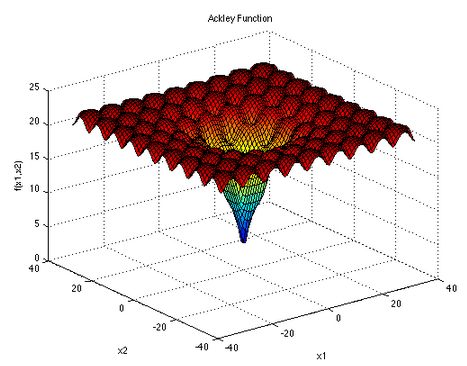
\includegraphics[width=0.27\textwidth]{../imagenes/ackley}
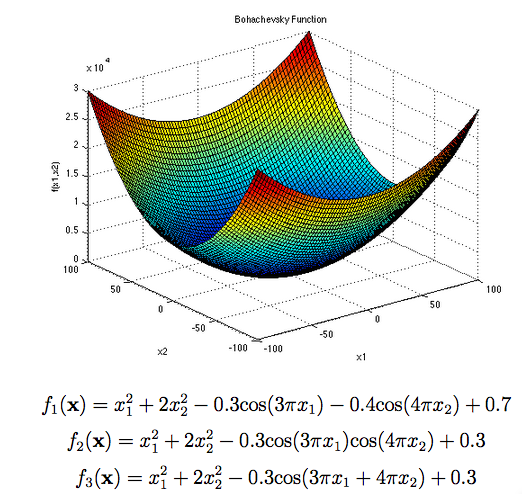
\includegraphics[width=0.27\textwidth]{../imagenes/boachevsky3}
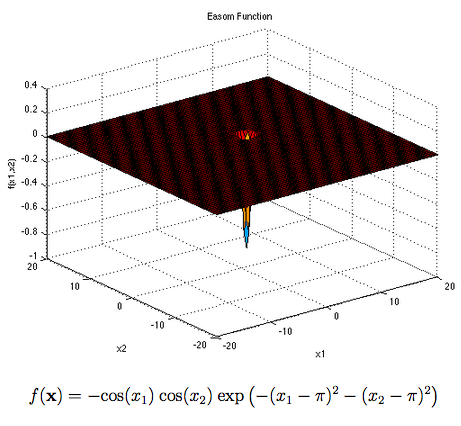
\includegraphics[width=0.27\textwidth]{../imagenes/easom}
\caption{De izquierda a derecha las funciones de Ackley, Boachevsky3 y Easom}
\end{figure}
\begin{figure}[ht]
\centering
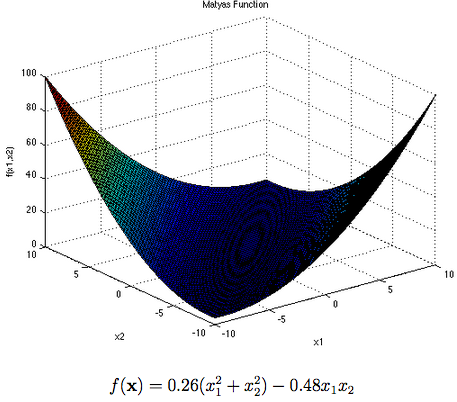
\includegraphics[width=0.27\textwidth]{../imagenes/matyas}
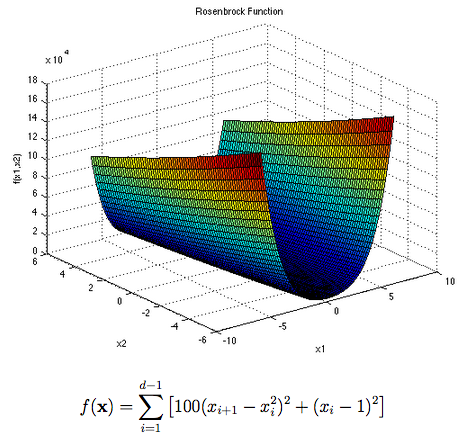
\includegraphics[width=0.27\textwidth]{../imagenes/rosenbrock}
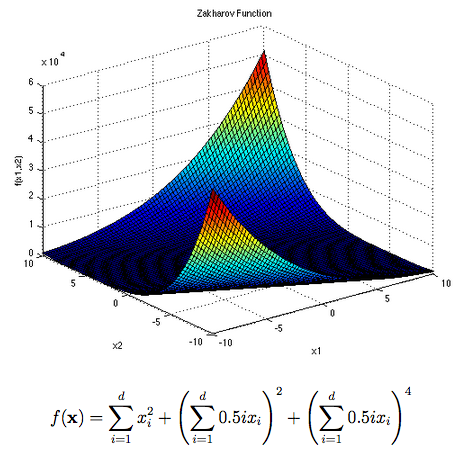
\includegraphics[width=0.27\textwidth]{../imagenes/zakharov}
\caption{De izquierda a derecha las funciones de Matyas, Rosenbrock y Zakharov}
\end{figure}
\begin{figure}[ht]
\centering
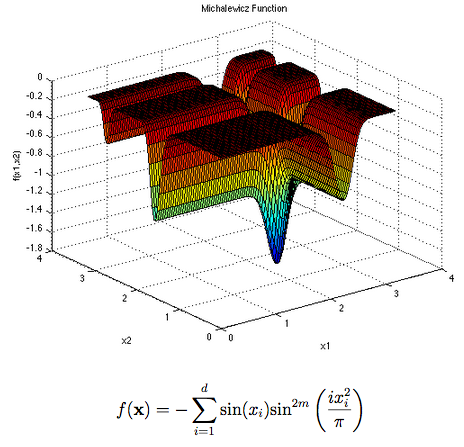
\includegraphics[width=0.27\textwidth]{../imagenes/mixhalewicz}
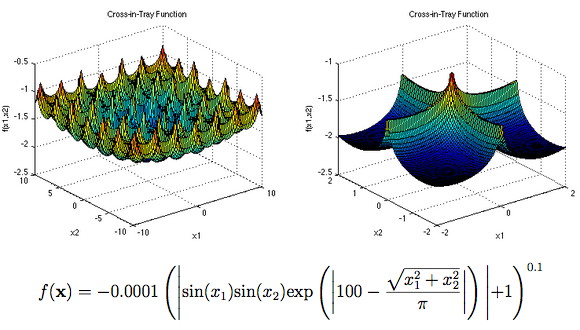
\includegraphics[width=0.45\textwidth]{../imagenes/crosstray}
\caption{De izquierda a derecha las funciones de Mixhalewicz y Crosstray}
\end{figure}
\begin{figure}[ht]
\centering
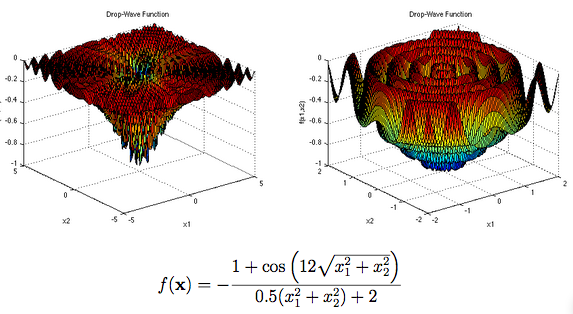
\includegraphics[width=0.45\textwidth]{../imagenes/dropwave}
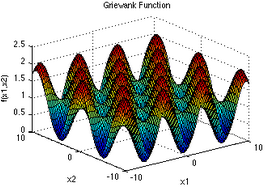
\includegraphics[width=0.45\textwidth]{../imagenes/griewank}
\caption{De izquierda a derecha las funciones de Drop-Wave y Griewank}
\end{figure}

\newpage

\section{Desarrollo del Experimento}

\subsection{Estructura del Programa}
El programa comienza con el \texttt{lanzador.R} que actúa como orquestrador. Desde aquí se llama al \texttt{inicializador.R}, que inicializa los datos de las funciones a resolver del directorio \texttt{funciones}; y se realiza un bucle que va llamando a la función en \texttt{evolutivo.R}, que contiene el algoritmo evolutivo; resolviendo todas las instancias de los problemas a resolver.

Dentro de \texttt{evolutivo.R} hay una función que va llamando a todas las subrrutinas que componen el algoritmo tal y como está descrito en el artículo \cite{mainPaper} y la primera sección de este informe. Los scripts que contienen estas subrrutinas son:

\begin{enumerate}
    \item \texttt{mutacion.R}: este script recibe como argumento una población de individuos y genera una lista de mutaciones, sin modificar la población original.
    \item \texttt{crossover.R}: este script toma la población original y la lista de mutaciones de \texttt{mutacion.R} y las combina generando un nuevo individuo \textit{trial}, en base a la variable \textit{CR}, que determina la probabilidad de un individuo de mutar.
    \item \texttt{seleccion.R}: este script selecciona los individuos eligiendo entre los individuos originales y los \textit{trials}. Para ello tiene en cuenta el \textit{fitness} de los individuos y el \textit{fitness ponderado} (\ref{ec_fitness_ponderado}) que se calcula desde \texttt{fitnessPonderado.R}. Devuelve una lista ordenada por \textit{fitness} de la nueva población.
    \item \texttt{fitnessPonderado.R}: Evalua la expresión (\ref{ec_fitness_ponderado}) sobre la población y devuelve sus \textit{fitness ponderado}.
    \end{enumerate}

\subsection{Parámetros del Algoritmo}
En este experimento existen tres parámetros que el usuario debe prefijar desde el principio y no se modifican por el algoritmo, que son $\xi_{1}=$, $\xi_{3}$ y $F_{2}$. Aquí hemos utilizado los mismos que en el artículo \cite{mainPaper}, es decir, $\xi_{1}=0.05$, $\xi_{3}=0.05$ y $F_{2}=0.5$.

En el artículo se sugiere que el valor de $\xi_{1}$ se puede incrementar hasta 0.2 para problemas complicados. No obstante aquí hemos mantenido los parámetros del artículo, ya experimentando con pequeños ajustes no hemos obtenido cambios significativos en el comportamiento del algoritmo para los problemas seleccionados.

Además hemos para cada problema el algoritmo se ha repetido 25 veces y se ha tomado una población inicial aleatoria de 1000 individuos. 

\section{Resultados y Conclusiones}
En la siguiente tabla se muestran los resultados obtenidos para los distintos problemas, incluyendo el tiempo de ejecución. En la columna ``Error'' se muestra la diferencia absoluta entre la mejor función objetivo y el mínimo de la función (ver la tabla de la sección~\ref{sec_tablaFunciones}).

\[\arraycolsep=7pt\def\arraystretch{1.4}
\begin{array}{|c|c|c|c|c|}
\hline
\text{\textbf{Problema}} & \text{\textbf{Mejor F.Obj.}} & \text{\textbf{Error}} & \text{\textbf{Mediana F.Obj.}} & \text{\textbf{Tiempo 25 ejec.}} \\ \hline
\text{Ackley} & 0.0 & 0.0 & 0.020933 & 71.342 \\ \hline
\text{CrossInTray} & -2.062612 & 0.0 & -2.062612 & 60.682 \\ \hline
\text{Drop-Wave} & -1.0 & 0.0 & -0.936245 & 59.009 \\ \hline
\text{Griewank} & 0.0 & 0.0 & 1e-0.6 & 123.424 \\ \hline
\text{Bohachevsky3} & 0.0 & 0.0 & 2.11502 & 57.581 \\ \hline
\text{Matyas} & 0.0 & 0.0 & 0.000102 & 56.372 \\ \hline
\text{Zakharov} & 0.0 & 0.0 & 5.9e-5 & 70.644 \\ \hline
\text{Rosenbrock (1)} & 0.0 & 0.0 & 1.689961 & 70.063 \\ \hline
\text{Rosenbrock (2)} & 0.0 & 0.0 & 0.0 & 62.868 \\ \hline
\text{Michalewicz (2D)} & -1.716269 & 0.085031 & -0.540872 & 73.296 \\ \hline
\text{Easom} & -0.998611 & 0.001389 & -0.005659 & 62.741 \\ \hline
\end{array}\]

\subsection{Mediana vs.\ media}
En los resultados mostrados al comienzo de esta sección se utiliza la mediana en lugar de la media. Para explicar esta elección, veamos como ejemplo un extracto de las ejecuciones sobre la función Ackley:
\begin{table}[hb]
\centering
\begin{tabular}{cc}
    Num.\ ejecución & Función objetivo\\\toprule
    15&0.000000\\
    16&0.000141\\
    17&16.46224\\
    18&0.095270\\
    19&0.000000\\
\end{tabular}
\end{table}

De forma intuitiva descartamos la ``explosión'' de la ejecución número 17, ya que es dos órdenes de magnitud mayor que el resto. Este efecto es aún más notable cuando, de las 25 ejecuciones, solo hay dos con un fitness mayor a 0.1. Estas explosiones son comunes al optimizar las funciones benchmark, que están diseñadas con el objetivo de ofuscar algoritmos de optimización.

Las explosiones hacen de la media una herramienta inútil. Siguiendo con las 5 ejecuciones del ejemplo, al hacer la media obtenemos que es $\approx 5.3$, esencialmente una quinta parte de la ejecución 17. La mediana, por otra parte, tiene un valor de 0.000141, mucho más acorde a los resultados. En resumen: la mediana nos permite filtrar las explosiones mientras que en la media contamina todas las medidas.

\subsection{Conclusiones}
Si miramos los valores de la mediana veremos que para la mayoría de los problemas está bastante cercana al mínimo de su problema, con varias excepciones como el Bohachevsky o el Michalewicz.

Si atendemos a los valores de la mejor función objetivo, veremos que todos los valores están a menos de una décima de distancia y la mayoría tienen el valor de la función en el mínimo (precisión de 6 decimales). Esto es un muy buen resultado, ya que nos indica que el algoritmo es capaz de llegar al mínimo de la función. Es muy probable que, adaptando el algoritmo (p.e.\ modificando las $\xi_i$), el algoritmo encontrase el mínimo absoluto, mejorando consecuentemente la mediana.
\vspace{1cm}

Este algoritmo de evolución diferencial ha demostrado una gran versatilidad, siendo capaz de resolver la mayoría de las funciones benchmark descritas en la sección~\ref{sec_funciones} tras 25 ejecuciones. Para aquellas que no ha conseguido resolver con la precisión deseada ---i.e.\ las funciones Michalewicz y Easom--- el error no es demasiado alto, y suponemos que una selección cuidadosa de los parámetros $\xi_i$ podría mejorar mucho estos casos particulares.
\vspace{5cm}

\bibliography{bibliografia}{}
\bibliographystyle{ieeetr}

\newpage

\section{Anexo. Código del programa} 

\subsection{lanzador.R}
\lstinputlisting{../lanzador.R}
\subsection{inicializador.R}
\lstinputlisting{../inicializador.R}
\subsection{evolutivo.R}
\lstinputlisting{../evolutivo.R}
\subsection{fitnessPonderado.R}
\lstinputlisting{../fitnessPonderado.R}
\subsection{mutacion.R}
\lstinputlisting{../mutacion.R}
\subsection{crossover.R}
\lstinputlisting{../crossover.R}
\subsection{seleccion.R}
\lstinputlisting{../seleccion.R}
\end{document}
